

\section{Introduction}
\label{sec:corpusCreation.introduction}

\todo{Add scintillating introduction.}


\todo{ Computational social science runs on twitter data.
7.7M google scholar results for twitter, with over 140k in just 2022.
How many of these studies query for a hashtag or keyword to build a corpus?
How many would benefit from training a classifier to filter out irrelevant tweets?}

The wide-spread availability of social media data
has resulted in an explosion of social science studies
as researchers adjust
from data scarcity
to abundance
in the internet age~\cite{lazer2009computational,lazer2021meaningful}. 

\todo{Analysis of social media data promises to supplement
traditional polling methods
by allowing for
rapid, near real-time measurements
of public opinion,
and allowing for historical studies of public language.
Polling remains the gold standard
for measuring public opinion where precision matters, ~\cite{cody2015climate} } 



\todo{Question}


When researchers characterize online discourse around a specific topic, a few approaches are available.
Each comes with trade-offs, both in researchers' time as well as the resulting precision and recall of the corpus.

Querying for relevant hashtags,
which signal an author's intent to attach their post to broader topic,
can match with relevant posts with high precision,
but often low recall.  
Hashtag based queries have been used by researchers
to construct focused corpora of tweets ranging from sports and music~\cite{blaszka2012worldseries,choi2014south},
to natural disasters, political activism, and
protests~\cite{steinert2015online,lotan2011arab,freelon2016beyond,jackson2020hashtagactivism,gallagher2019reclaiming,gallagher2018divergent,gorodnichenko2021social,arnold2021hurricanes}.

Alternatively, researchers can query for posts with an expansive set of keywords
to increase recall at the expense of precision. 
Expanding this set of keywords can be done with by experts with domain expertise, algorithmically, or a combination.
Broad expert crafted keyword lists have been used to study
social responses to the COVID-19 pandemic~\cite{shugars2021pandemics,chen2020tracking,green2020elusive,twitter_2020}\todo{Add more examples here?}.
Other researchers have used algorithmically generated lists of keywords,
by comparing the distribution of words in a corpus of interest to a reference corpus and selecting words with high rank-divergence contributions~\cite{dodds2020allotaxonometry,alshaabi2021world,minot2022distinguishing,stupinski2022quantifying}. 
But continued expansion beyond the most relevant keyword necessarily reduces precision. 
Researchers can further refine the set of relevant keywords to balance precision and recall,
or add complexity to their queries with negation or Boolean operators to require multiple keywords.

While some social media datasets can be sufficiently curated
with simple heuristics
or rules-based classifiers,
others could benefit from an alternative paradigm.
We argue for a two step pre-processing pipeline
that combines broad,
high recall keyword queries
with fine-tuned,
transformer-based classifiers
to increase precision.
This approach can trade the labor costs associated with building rules-based filters, 
for the cost of labeling social media data for few-shot learning~\cite{wang2020generalizing}, while still achieving high precision.

Since the introduction of Word2Vec in 2013 and GloVe in 2014,
the natural language processing community has had access to high quality, global word embeddings~\cite{mikolov2013efficient,pennington2014glove}.
These embeddings are trained vector representations of words from given a corpus of text,
enabling word comparisons with distance metrics.
However, global embeddings will average the representations of words,
making them unsuitable for document classification
where key terms have multiple meanings.
The development of attention  %~\cite{joulin2017bag} ~\cite{vaswani2017attention}
\todo{More about transformers}

\todo{specifically about sentence embeddings, including different ones we tried}. 
While transformer based language models like BERT provide state of the art performance on natural language processing tasks, they are computationally expensive to run. Creating sentence embeddings with Siamese, transformer networks, promises large improvements in computational efficiency for sentence classification, while maintaining state-of-the art performance~\cite{reimers-2019-sentence-bert}.

\todo{text classification for longer texts has been less successful \cite{gao2021limitations}. Text classification with a large number of classes is also challenging }\cite{gao2021limitations}\cite{chang2020taming}


\todo{more of classifying tweets}~\cite{antypas2022twitter} ~\cite{quercia2012tweetlda}


Today, sophisticated, pre-trained language models are readily accessible to researchers through ~\cite{wolf2020transformers}, and can be easily fine-tuned with a limited amount of labeled data, so ~\cite{yan2018few,wang2020generalizing}

\todo{more on renewable energy specifically}
\cite{kim2020exploring, jain2019sentiment}


Although we focus on the topic of renewable energy, we hope our methods are broadly applicable
to any text-based social media dataset.

\section{Methods and Data}
\label{sec:corpusCreation.methods}



We explore the performance of contextual sentence embedding based text classifiers for corpus curation through a selection of case studies. 


\subsection{Description of data sets}
\label{sec:corpusCreation.data}

In this study we examine ambient tweet datasets,
collections of tweets that are anchored by a single keyword or set of keywords. 
From Twitter's Decahose API,
a 10\% sample of all tweets,
we begin by selecting tweets containing valid user-provided locations in the United States. 
From this selection, we query for tweets that both contain keywords of choice and are classified as English by FastText~\cite{joulin2017bag}.
We define the results of this query as the unfiltered ambient corpus.

We chose three keywords related to non-fossil fuel energy generating technologies, \texttt{`Wind'}, \texttt{`Solar'}, and \texttt{`Nuclear'}. 
Over the study period from 2016 to 2022, these keywords matched 3.43M, 1.39M, and 1.29M tweets in our subsample, respectively.

While the terms of service with Twitter do not allow us to publish raw tweets, we provide relevant tweet IDs for rehydration. 
\todo{Add tweet\_id extractor to git repo.}

\subsection{Relevance classification}
For classification we hand-labeled a random sample of 1000 matching tweets
for each keyword
as either `relevant' (R)  or `not relevant' (NR) to energy production. 
We've made of tweet IDs and corresponding labels available for both the training data 
as well as predicted labels for the full dataset.
\todo{add this}

We trained three models for comparison,
two contextual sentence embeddings, \texttt{all-mpnet-base-v2} and \texttt{all-MiniLM-L6-v2},
and one non-contextual model, created by averaging \texttt{GloVe} word embeddings. 
We've listed the performance of the models in Tabel~\ref{tab:F1-scores}.

\todo{Add some more model F1 scores, maybe a for L6, and for Glove if you can do it with Hugging Face, else go edit }

\begin{table}[t]
\begin{tabular}{lllll}
\toprule
   & Wind & Solar & Nuclear \\
     \cmidrule(lr){2-4} 

   \% Relevant & 4.7\% & 43.7\% & 16.0\% \\
F1 & 0.90 & 0.95  & 0.86   \\

  \bottomrule

\end{tabular}
\caption{}
\label{tab:F1-scores}
\end{table}



\subsection{Corpus Comparison}

\todo{Corpus comparison}








% Figure 1
\begin{figure*}
  \centerfloat	
        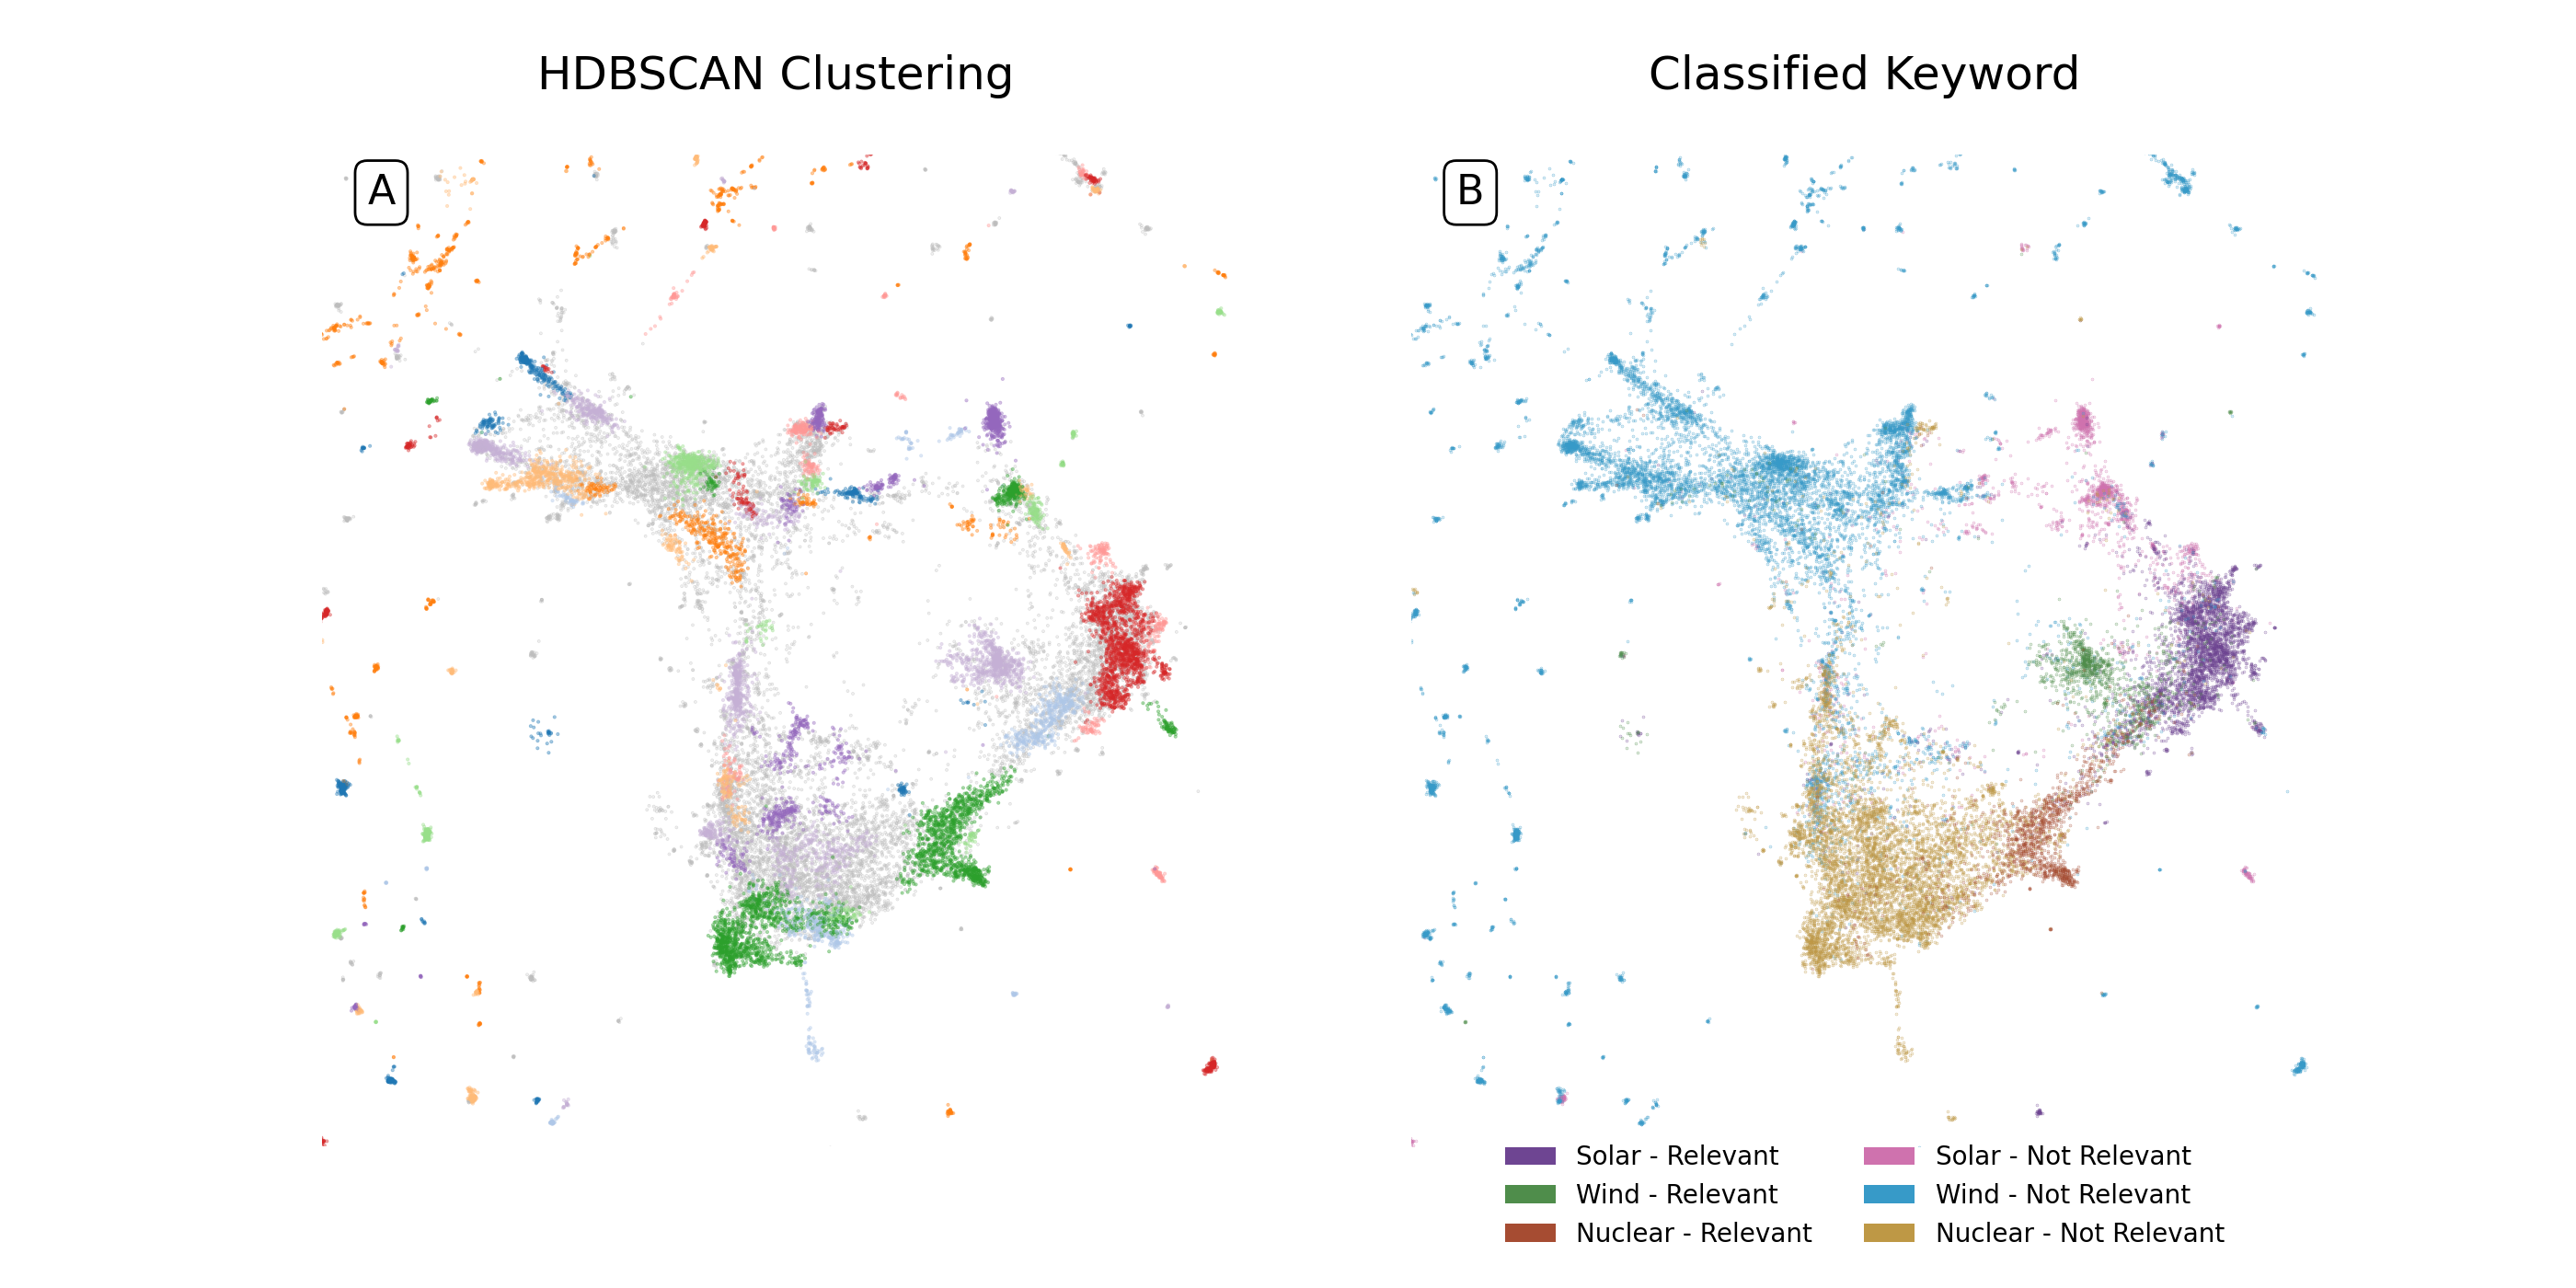
\includegraphics[width=2.8\columnwidth]{figures/combined_labeled_embedding_horizontal.png} 
  \caption{\textbf{Embedded tweet distribution plot} for the combined datasets.
  Using a pre-trained model for semantically meaningful sentence embeddings, \texttt{all-mpnet-base-v2}, we plot the distribution of tweets within this semantic space.
  In both plots points are tweets projected into 2D using UMAP for dimensionality reduction.
  In panel A, we perform density based, hierarchical clustering using HDBSCAN and color by cluster.
  In panel B, we color by both the keyword used to query and the classification as relevant or not relevant to the topic of clean energy. 
  Relevant tweets containing the keywords \anchor{wind}, \anchor{solar}, and, to a lesser extent, \anchor{nuclear} are relatively close together on the right in the embeddings, while not relevant tweets are more dispersed.} 
    \label{fig:combined_embeddings}
\end{figure*}


\subsection{}











\todo{Compare performance of contextual sentence embeddings to glove?}

\todo{Expand on fine-tuning and classification procedure.}






\section{Results}
\label{sec:corpusCreation.results}






\todo{Explain what we found}



\todo{Solar tweets were nearly evenly split with 47\% of the corpus being relevant and 53\% being not relevant by volume of words.}

\todo{plot of relevant vs non-relevant tweets in the embedding space.}
\todo{sentiment plot}




\begin{figure*}
  \centering	
    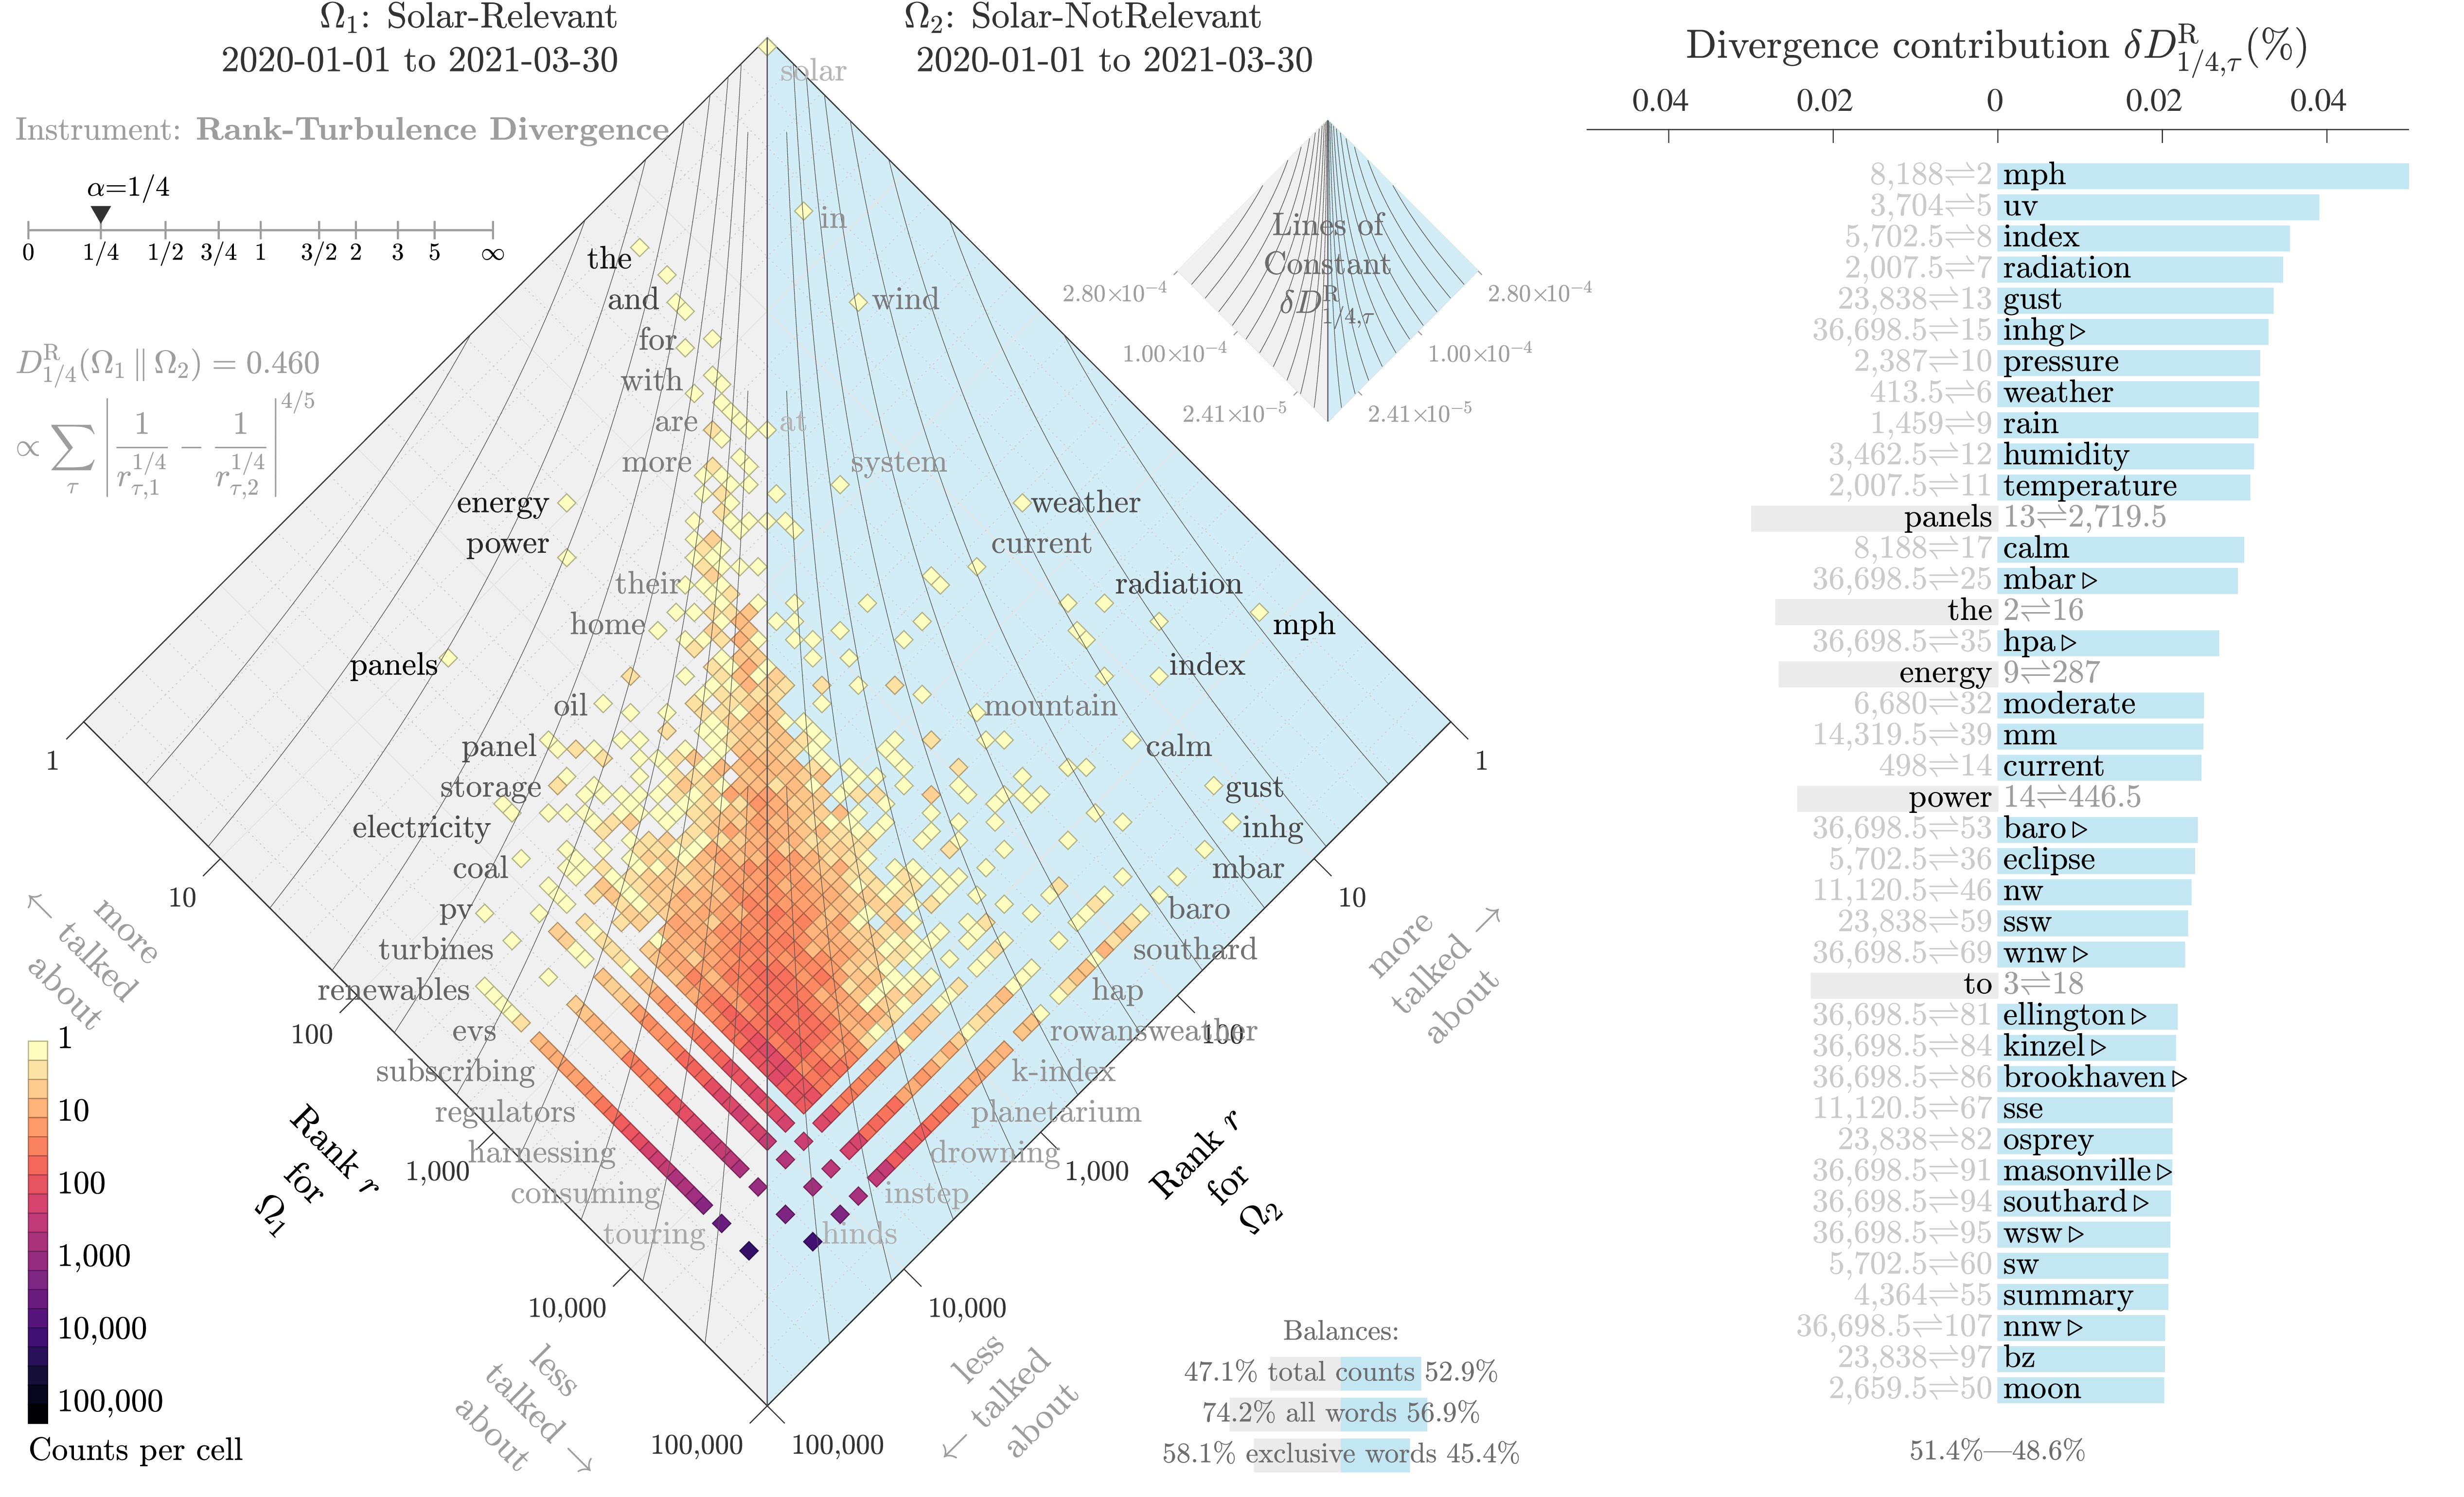
\includegraphics[width=0.90\textwidth]{figures/figallotaxonometer9000-2021-03-30-2021-03-30-rank-div-alpha-third-Solar_Solar_noname.png}  
  \caption{\textbf{Allotaxonograph comparing the rank divergence of words
    classified as relevant to solar energy discourse
    to those containing the keyword \anchor{solar}
    but classified as not relevant.} 
    On the main 2D rank-rank histogram panel,
    words appearing on the right have a higher rank in the ``relevant'' subset than in ``not relevant'', while phrases on the left appeared more frequently in the ``not relevant'' tweets.
    The panel on the right shows the words which contribute most to the rank divergence between each corpus.
    %% examples
    We observe that many words associated with weather bots,
    such as ``mph,'' ``uv,'' and ``pressure,'' 
    are more frequently used in non-relevant posts,
    while words like ``panels,'' ``energy,'' and ``power,'' used more in tweets relevant to solar energy.
    Notably, commonly used function words,
    such as ``the,'' ``and,'' and ``are,'' 
    are off-center in the rank-rank histogram, a further indication that many of the ``not relevant'' tweets are from automated accounts publishing weather data rather than using conversational English.
    The balance of the words in these two subsets is noted in the bottom right corner of the histogram, showing the percentage of total counts, all words, and exclusive words. 
    For this example the two subsets are nearly balanced, indicating that the filtered corpus contains less than 50\% of word tokens from the raw query.
    See Dodds~\etal~\cite{dodds2020allotaxonometry} for a full description of the allotaxonometric instrument.}
    \label{fig:rankdiv_solar}
\end{figure*}


\begin{figure}[tp!]
  \centering	
    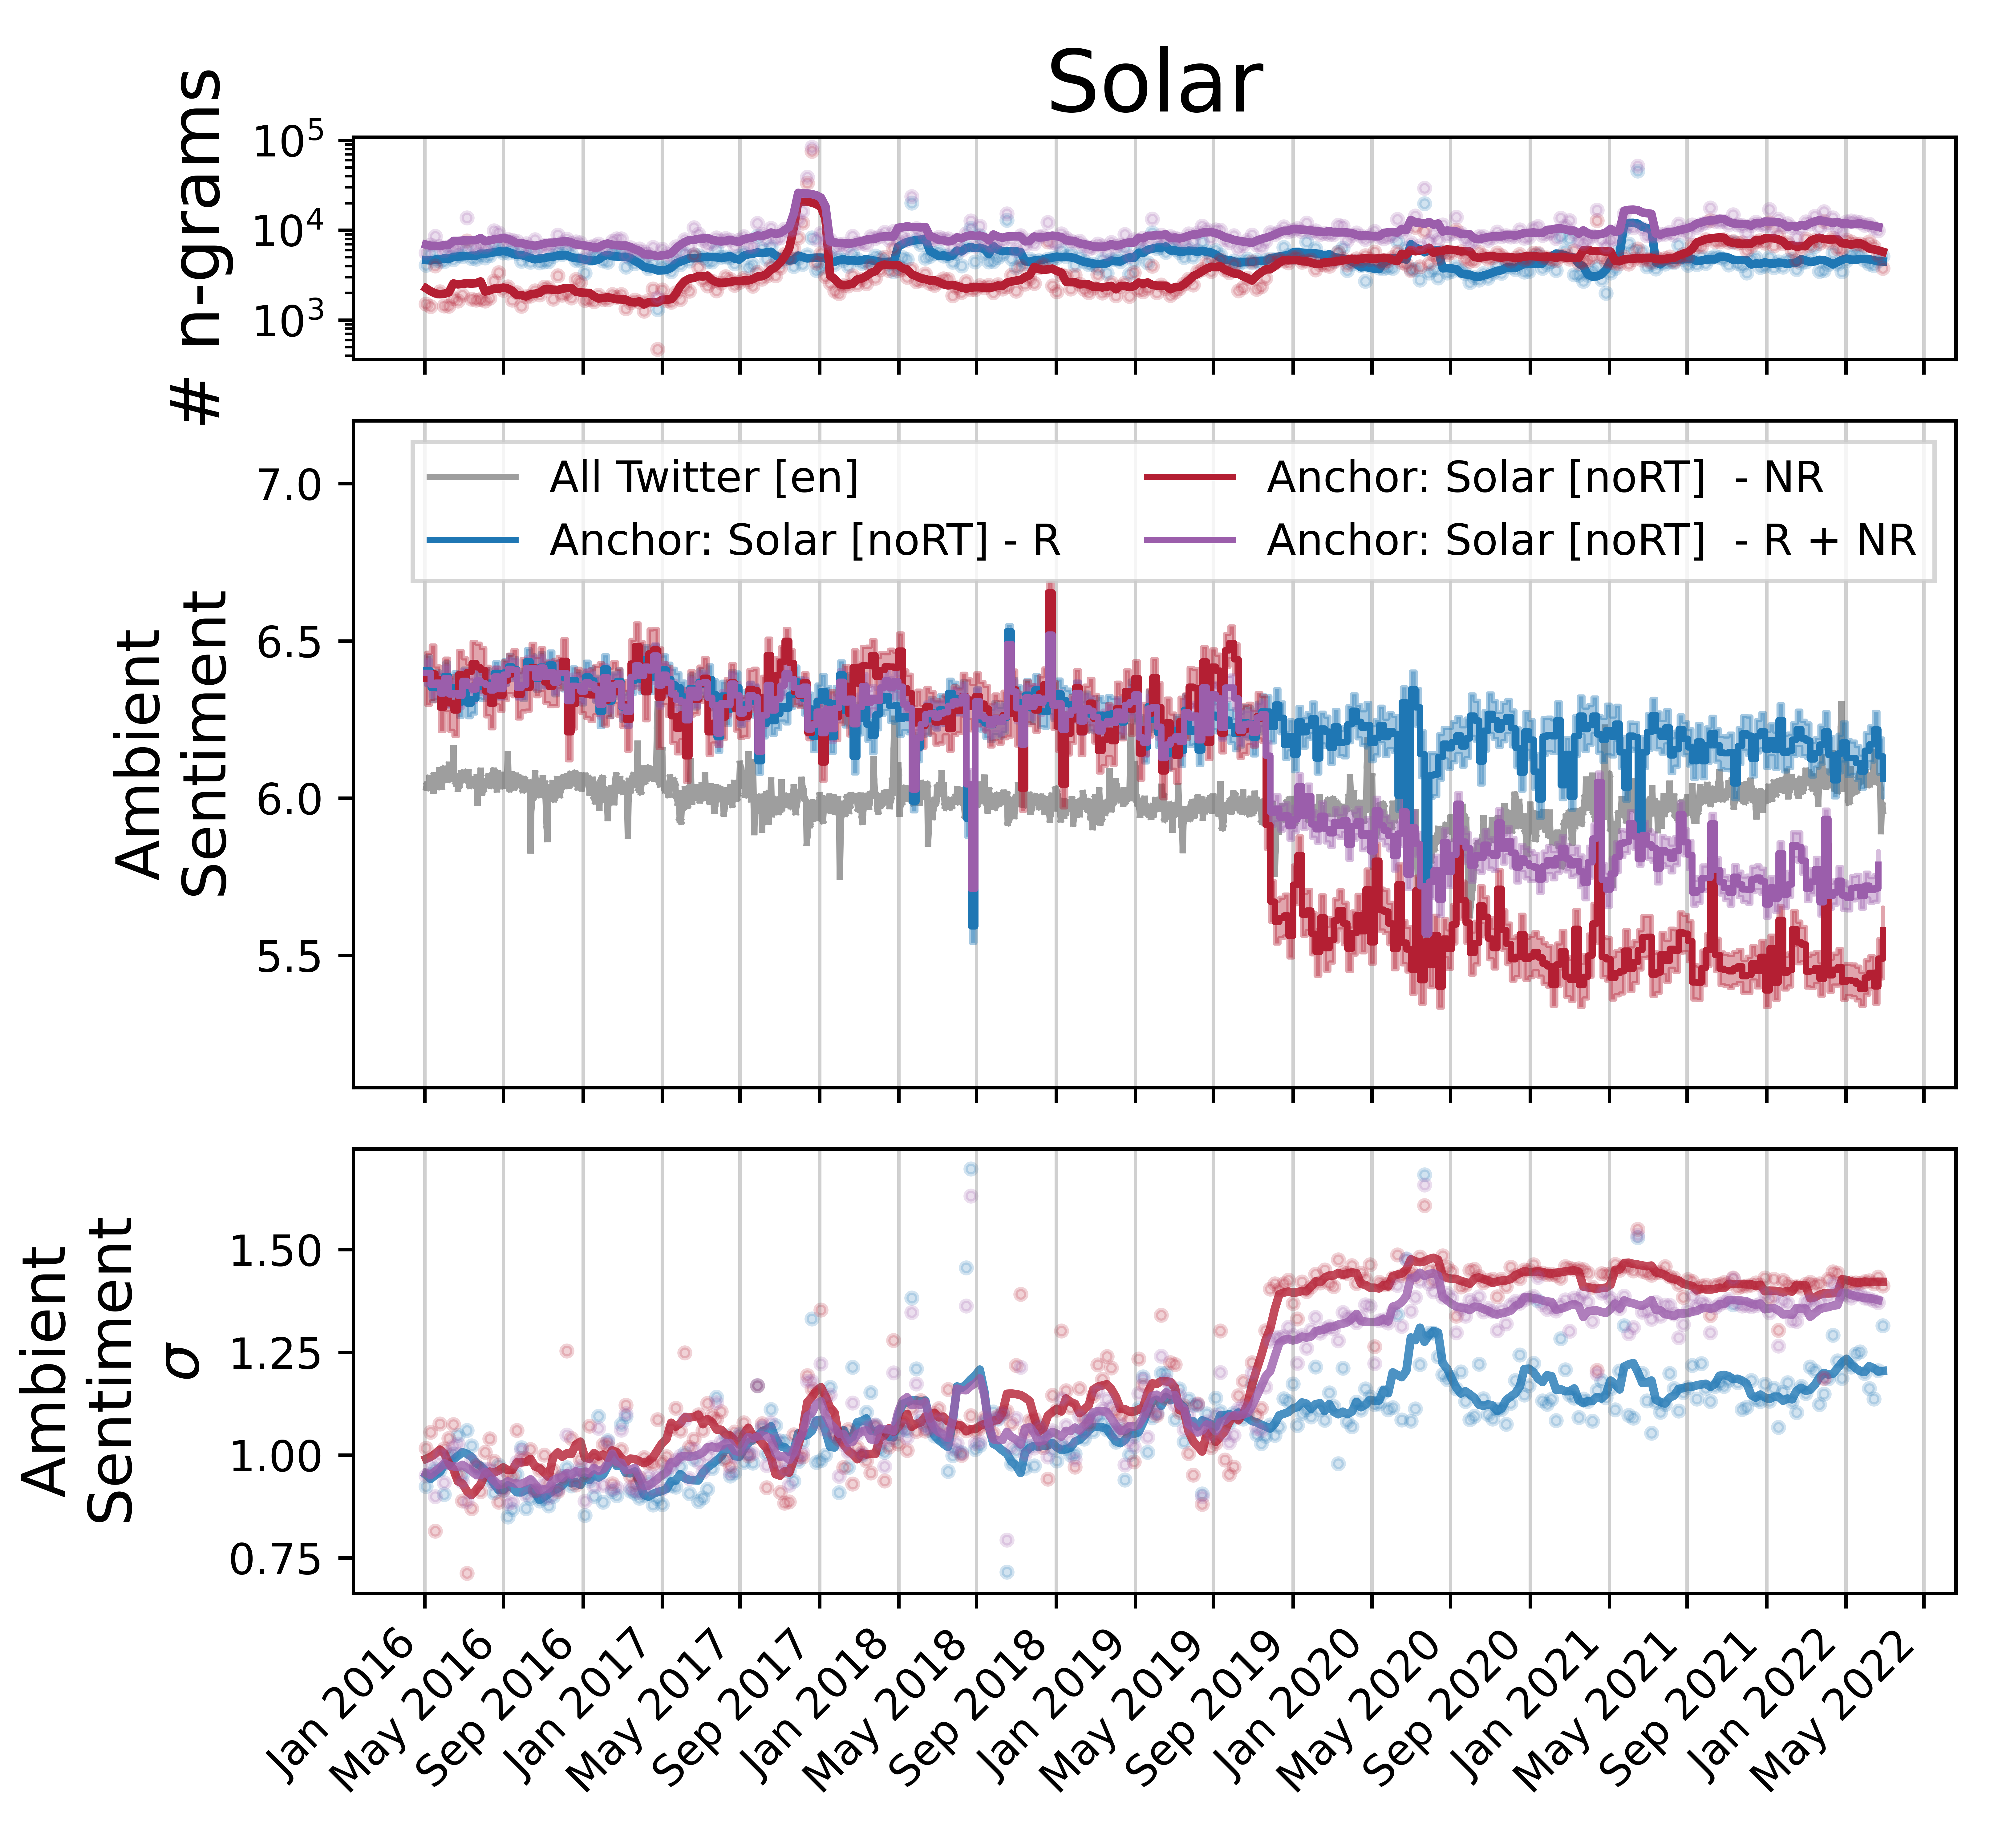
\includegraphics[width=0.98\columnwidth]{figures/Solar_sentiment_2016-01-01_2022-03-15.png}  
  \caption{
    \textbf{Ambient sentiment time series comparison for relevant  (R), non-relevant (NR), and combined tweet corpora, all containing the keyword \anchor{solar}.}
    In the top panel we show the number of tokens with LabMT \cite{dodds2015human} sentiment scores in each corpus on each day.
    `Relevant' tweets, in blue, have more scored tokens early on,
    but the number tokens in `not relevant' tweets increase in relative proportion over time.
    The center panel shows the average sentiment for each corpus, including measurement of English language tweets as a whole in gray for comparison. 
    Before 2019, the measured sentiment for both corpora are comparable, but later the mean sentiment of `non-relevant' tweets drops. 
    In the bottom panel we plot the standard deviation of the sentiment measurement, which captures a broader distribution of sentiment scores for  `non-relevant' tweets.
    Without classification filtering, the ambient sentiment measurement would been misleading, appearing as though the sentiment contained in tweets containing the word \anchor{solar} has dramatically dropped in 2019, when in fact sentiment has only modestly declined. 
  }
  \label{fig:solar_sentiment}
\end{figure}


\begin{figure*}
  \centering	
    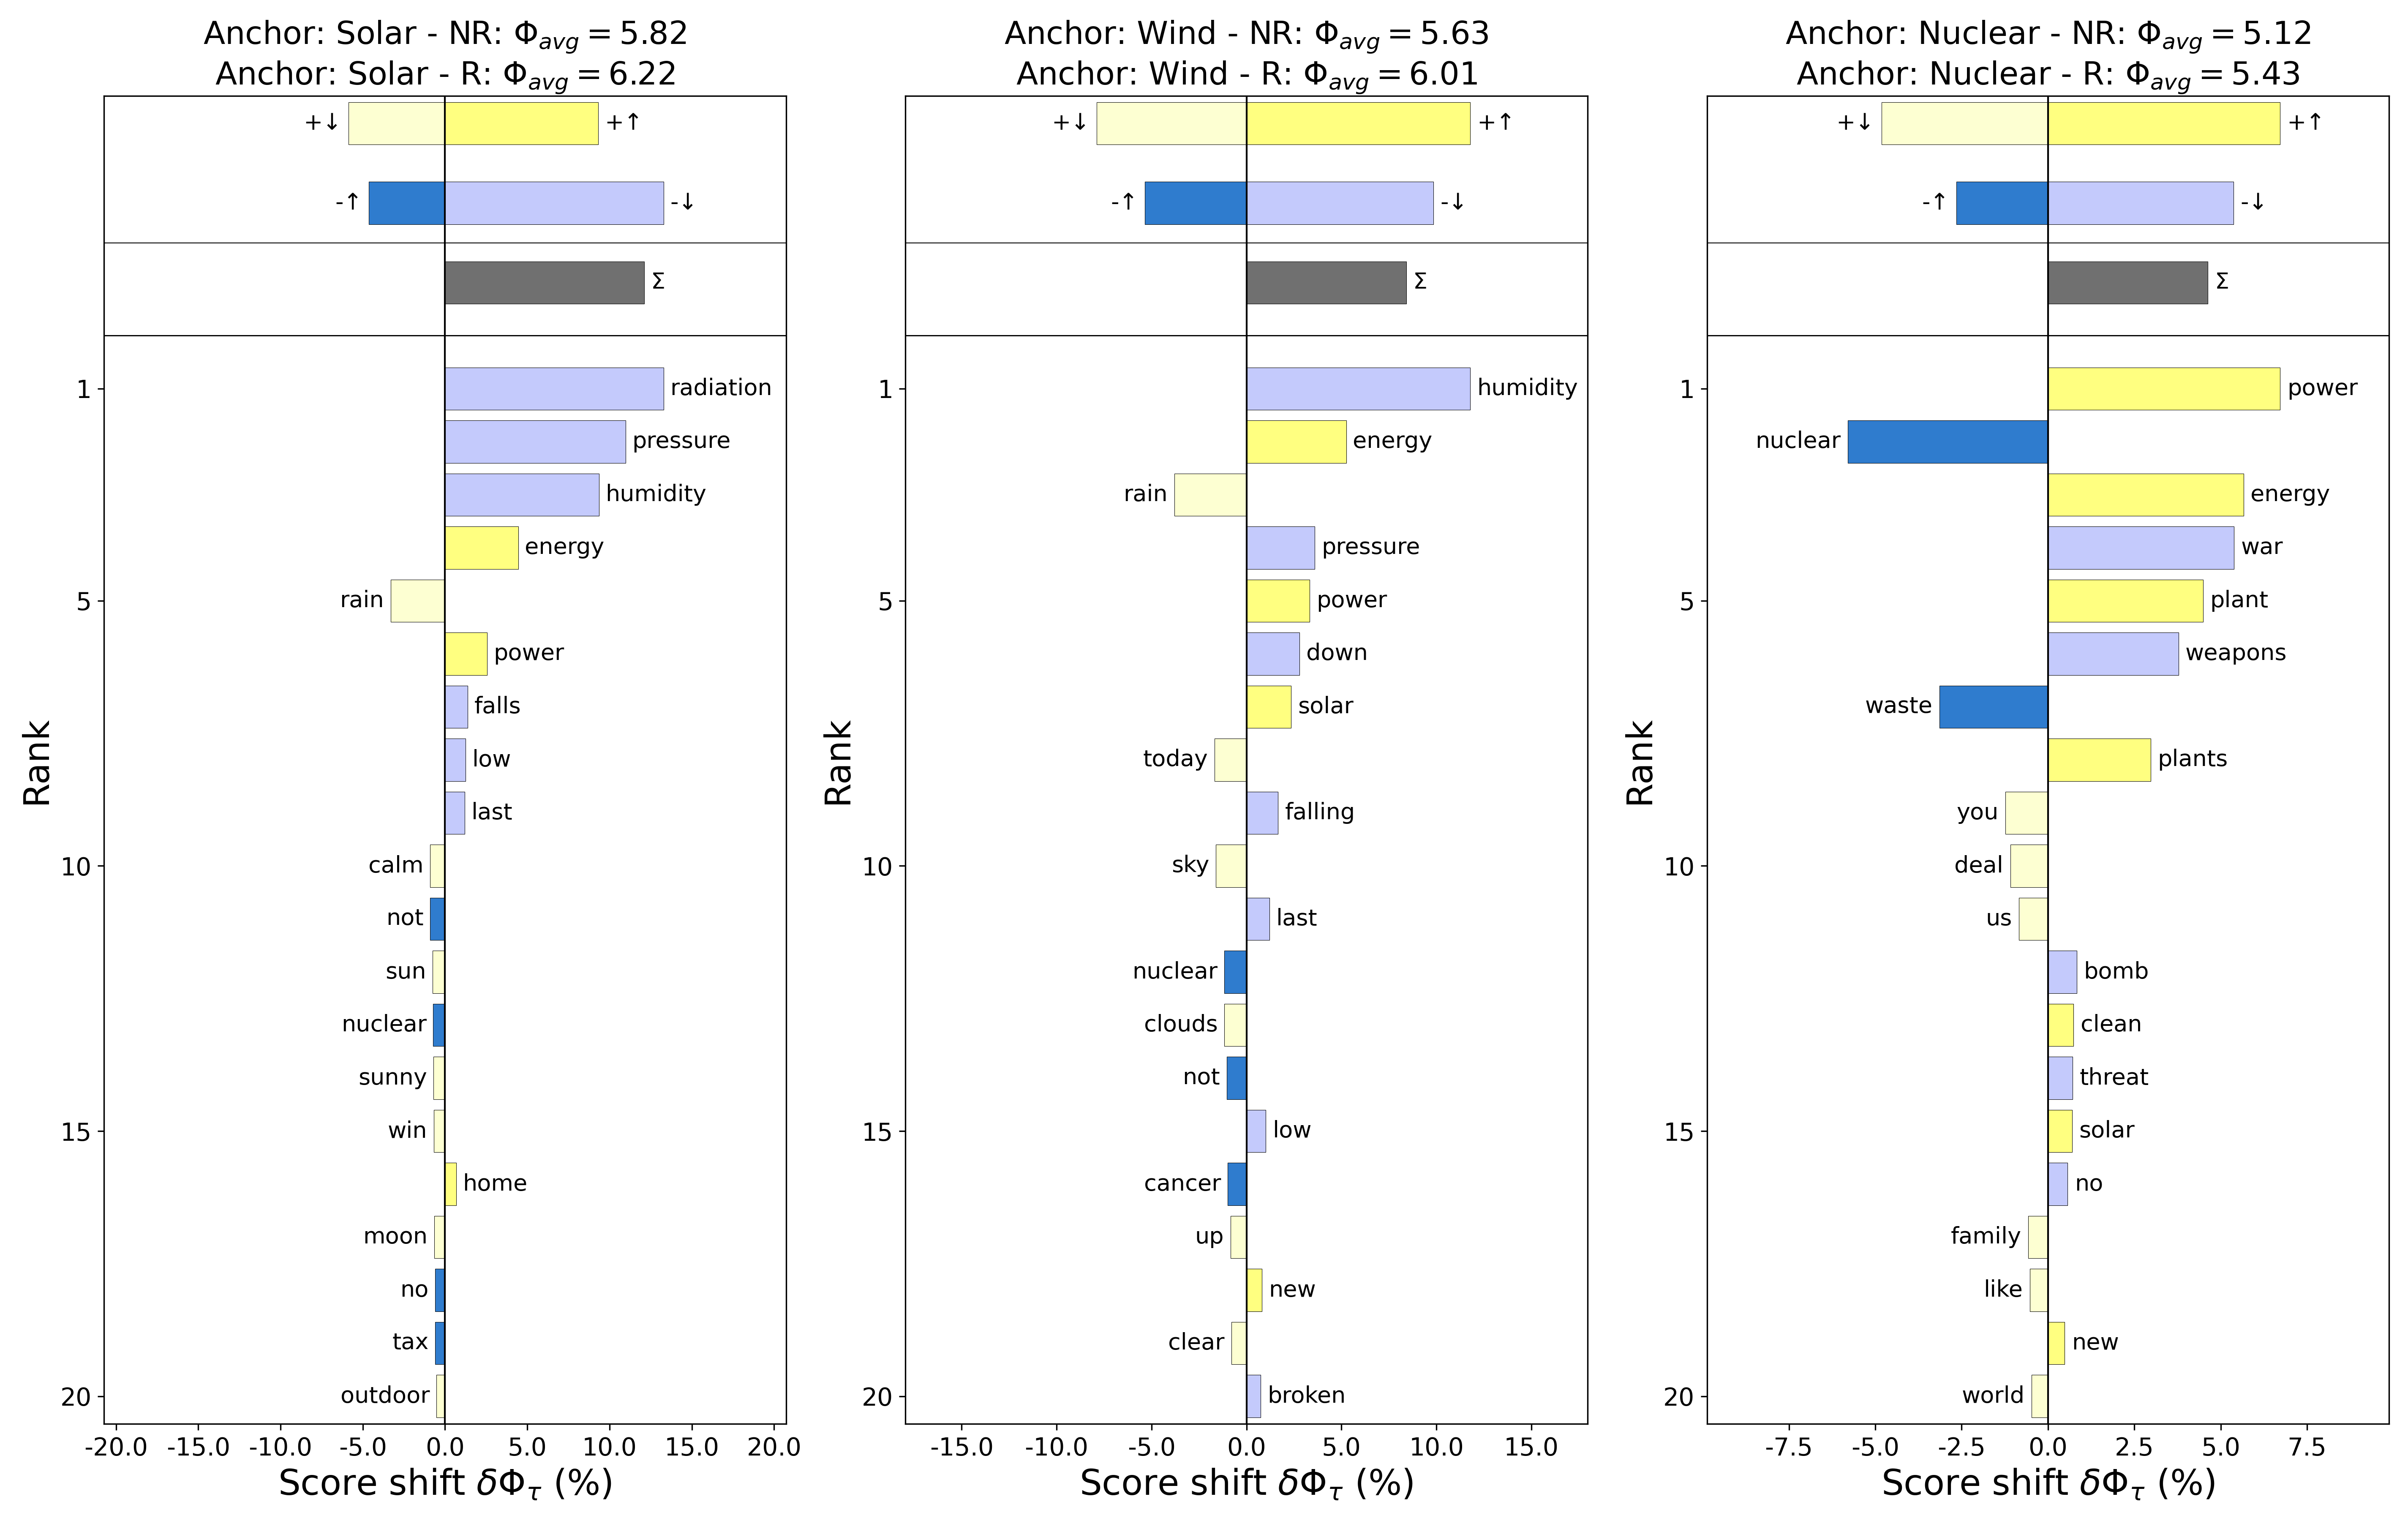
\includegraphics[width=0.98\textwidth]{figures/combined_shifts.png}  
  \caption{
    \textbf{Sentiment shift plots comparing the classified `relevant' (R) and `non-relevant' (NR) tweet corpora for tweets containing the keywords \anchor{solar}, \anchor{wind}, and \anchor{nuclear}.}
    We show the 20 top contributing words to the difference in LabMT sentiment between the corpora.
    `Relevant' tweets, those related to clean energy are happier on average for all keywords when compared to `not relevant' tweets. 
    Sad words that are less common in `relevant' \anchor{solar} tweets are `radiation', `pressure', and `humidity', which largely refer to the weather. Happy words like `energy' and `power' are more common in `relevant' tweets compared to tweets not relevant to solar energy. For \anchor{wind} sad terms like `humidity' and `pressure' are less common in `relevant' tweets, while happy terms like `energy', `power', and `solar' are more common in tweets relevant to wind as a renewable energy source. For \anchor{nuclear}, relevant tweets are on average more positive due to sad words like `war', `weapons', and `bomb' are less common in relevant tweets, while happy words like `power' and `energy' are more common. Some sad words like `nuclear' and `waste' do occur more frequently in relevant tweets.
  }    
  \label{fig:combined_sentiment_shifts}

\end{figure*}



\subsection{Solar energy case study}
\label{sec:corpusCreation.results.solar}

Of the three case studies 
we found the R \anchor{solar} tweets corpus evolved
most relative to the corresponding NR corpus.
Looking at the sentiment timeseries in \ref{fig:solar_sentiment}, 
we see little difference between the ambient sentiment of the R and NR corpora prior to 2019,
before NR ambient sentiment, shown in red, sharply falls as the R corpus appears to remain on trend.
For the standard deviation of ambient sentiment, 
which measures how broad is the distribution of sentiment scores for each LabMT word in the ambient corpus,
we also observe a dramatic increase in 2019.

We contend that the process of selecting relevant social media documents to include in a corpus
is just as important as the NLP measurement tools
used to quantify sentiment.
The difference in resulting sentiment measurement,
between what would have been measured without a classifier
(the R + NR corpus in purple) 
and the improved measurement after filtering with a classifier 
(the R corpus in blue) 
is stark. 
Looking at only the combined R + NR measurement,
researchers could incorrectly conclude that language surrounding \anchor{solar} has decreased dramatically since 2019. 

Focusing on only the R \anchor{solar} sentiment timeseries, it is clear that there was no dramatic drop in sentiment around \anchor{solar}, and this language remains more positive relative to Enlish language tweets in general.
\todo{sentiment timeseries}


\todo{sentiment shifts}
\todo{allotax}


\subsection{Wind Energy Case Study}
\todo{}
The unclassified \anchor{wind} tweets corpus had the lowest proportion of revelant tweets;
only 5\% of the human labeled subset was related to clean energy.
The n-gram \anchor{wind} is used in many different contexts besides energy generation,
from the weather to figurative uses like `second wind' and the phrase `wind up.' In the top panel of \ref{fig:wind_sentiment}, we can see that the number of n-grams with sentiment scores to make a measurement in the R corpus is consistant around $10^3$, while the NR corpus contain more than an order of magnitude more text.

We found the ambient sentiment of the R \anchor{wind} corpus has been slightly more positive than average language use on Twitter. 
\todo{whats going on with the negative spikes}
The NR corpus had distinctly lower sentiment, but was more dynamic, rising from a low of 5.5 in 2016, to 5.9 in 2020.
Because the proportion of tweets relevant to energy is so low, 
the combined sentiment time series measurement is dominated by the NR corpus. 
The standard deviation of sentiment, $\sigma$, for the R corpus also increased from around 1.0 in 2016, before leveling off around 1.2, slightly under the NR corpus.

\todo{write about using broad keywords, low precision keywords still being viable to create corpus with ML filtering}

\subsection{ Nuclear Energy Case Study}
\todo{}
The \anchor{nuclear} case study had the lowest classification performance after fine-tuning, 
acheiving an F1 score of just 0.86. 
The proportion of relevant tweets, 16\%, was higher than for the \anchor{wind} corpus, 
we believe the performance was impacted negatively by the close proximity 
of nuclear energy and nuclear weapons topics in the semantic space. 

The ambient sentiment timeseries for the R \anchor{nuclear} corpus was much lower than average sentiment on Twitter for then entire study period,
but higher than the NR corpus.

\section{Concluding remarks}
\label{sec:corpusCreation.concludingremarks}

\todo{Bring it home.}

\todo{limitations, not a representative sample, etc}
While our contribution


